\documentclass[10pt,a4paper]{article}
\usepackage[latin1]{inputenc}
\usepackage{amsmath}
\usepackage{amsfonts}
\usepackage{amssymb}
\usepackage{graphics}
\usepackage{hyperref}
\usepackage{fullpage}
\author{Gergely Imreh}
\title{Angular distribution after atomic beam collimator}
\begin{document}
\maketitle

\section{Distribution}
The aim of this calculation to derive the angular distribution of atoms after a pair of pinholes, just like the collimator tube before the Zeeman slower in our setup. The input and output pinholes have radius $r_1$ and $r_2$ respectively, they are assumed here to be concentric and separated by $L$.

Using a geometric picture, the proportion of atoms escaping through the two pinholes is proportional to the overlapping area of the holes. Looking at different angular direction $\theta$ is equivalent to shift the centre of the wholes by
\begin{equation}
d = L \sin\theta.
\label{eq:centreshift}
\end{equation}
The geometry is shown on Fig. \ref{fig:overlapping}.

\begin{figure}[ht]
\centering
\resizebox{0.6\columnwidth}{!}{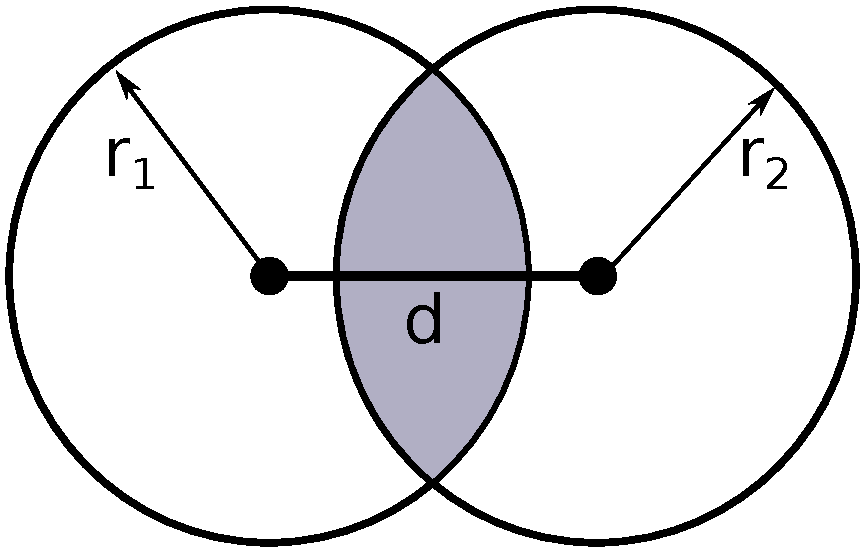
\includegraphics{overlapping.pdf}}
\caption{Overlapping circles geometry, $r_1$ and $r_2$ are the radius of the input and output pinholes, respectively. The difference of their centres $d$ is defined according to Eq. \ref{eq:centreshift}.}
\label{fig:overlapping}
\end{figure}


The overlapping area can be calculated as \footnote{See on MathWorld: \url{http://mathworld.wolfram.com/Circle-CircleIntersection.html}}:
\begin{eqnarray}
A(\theta, r_1, r_2, L) &=& r_1^2 \cos^{-1}\left(\frac{d^2+r_1^2-r_2^2}{2 d r_1}\right) + \nonumber\\
  & & r_2^2 \cos^{-1}\left(\frac{d^2+r_2^2-r_1^2}{2 d r_2}\right) - \nonumber\\
  & & \frac{1}{2} \sqrt{(-d+r_1+r_2)(d+r_1-r_2)(d-r_1+r_2)(d+r_1+r_2)}
\label{eq:overlaparea}
\end{eqnarray}
Taking into account that the angular distribution at the first pinhole is proportional to $\cos(\theta)$, and the number of atoms are normalized by the incoming number (i.e. the area of the first pinhole) the overall probability is
\begin{equation}
p(\theta) = A(\theta, r_1, r_2, L) \cos\theta / \pi r_1^2
\label{eq:angleprop}
\end{equation}
and the total proportion of atoms leaving the collimator at an angle $\theta \in [\alpha, \beta]$ is
\begin{equation}
P(\theta\in[\alpha, \beta]) = \frac{A(\hat \theta, r_1, r_2, L)}{\pi r_1^2} \int_{\alpha}^{\beta}\cos\theta d\theta 
                   = \frac{A(\hat \theta, r_1, r_2, L)\left(\sin\beta - \sin\alpha\right)}{\pi r_1^2} 
\label{eq:outprop}
\end{equation}
where $\hat \theta = (\beta + \alpha)/2$ and the $[\alpha,  \beta]$ range is assumed to be small.

To illustrate the behaviour of these functions, Fig. \ref{fig:entrysize} and \ref{fig:aspect} are showing the proportion of atoms escaping at a given angle when the entry pinhole size and the aspect ratio (i.e. collimator length) is changed, respectively, that is showing $p(\theta)/ \cos\theta$.

\begin{figure}[ht]
\centering
\resizebox{0.8\columnwidth}{!}{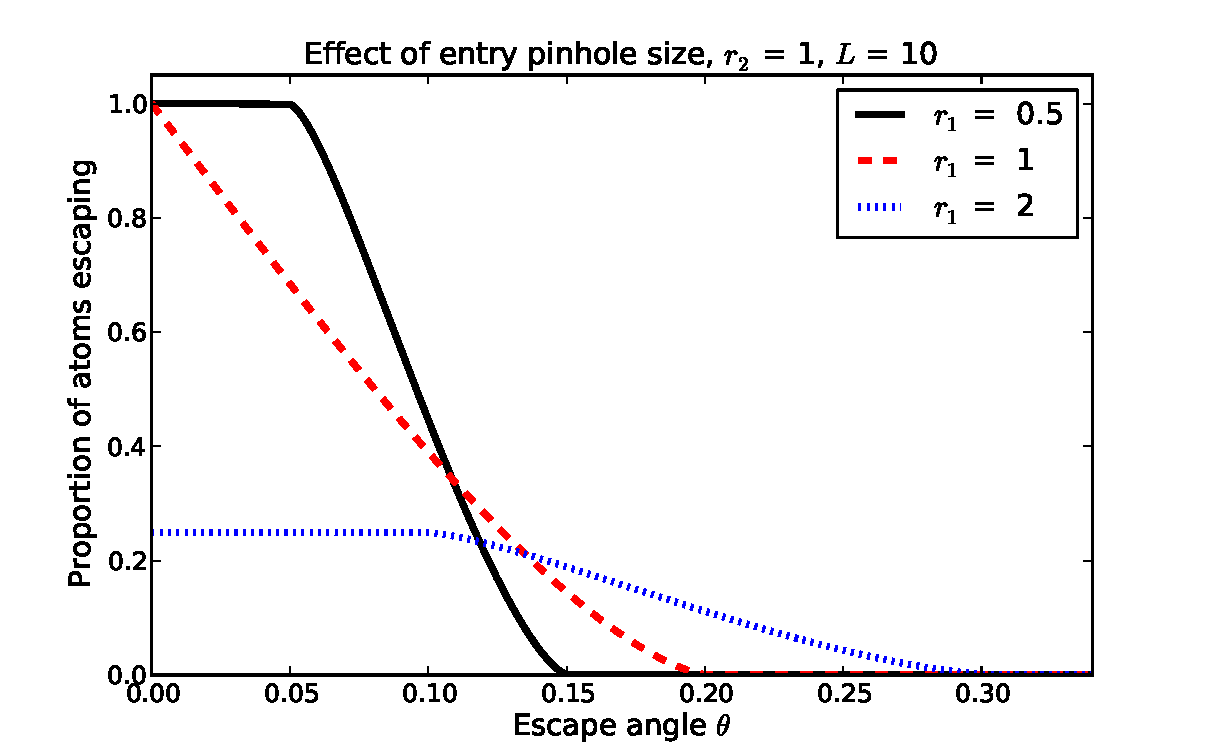
\includegraphics{pinhole_entrysize.pdf}}
\caption{The effect of entry pinhole size $r_1$ on the number of atoms escaping at different angles. The proportions are normalized by the number of atoms crossing the entry pinhole at that angle, i.e. 1 means all atoms that entered at angle $\theta$ managed to escape.}
\label{fig:entrysize}
\end{figure}

\begin{figure}[ht]
\centering
\resizebox{0.8\columnwidth}{!}{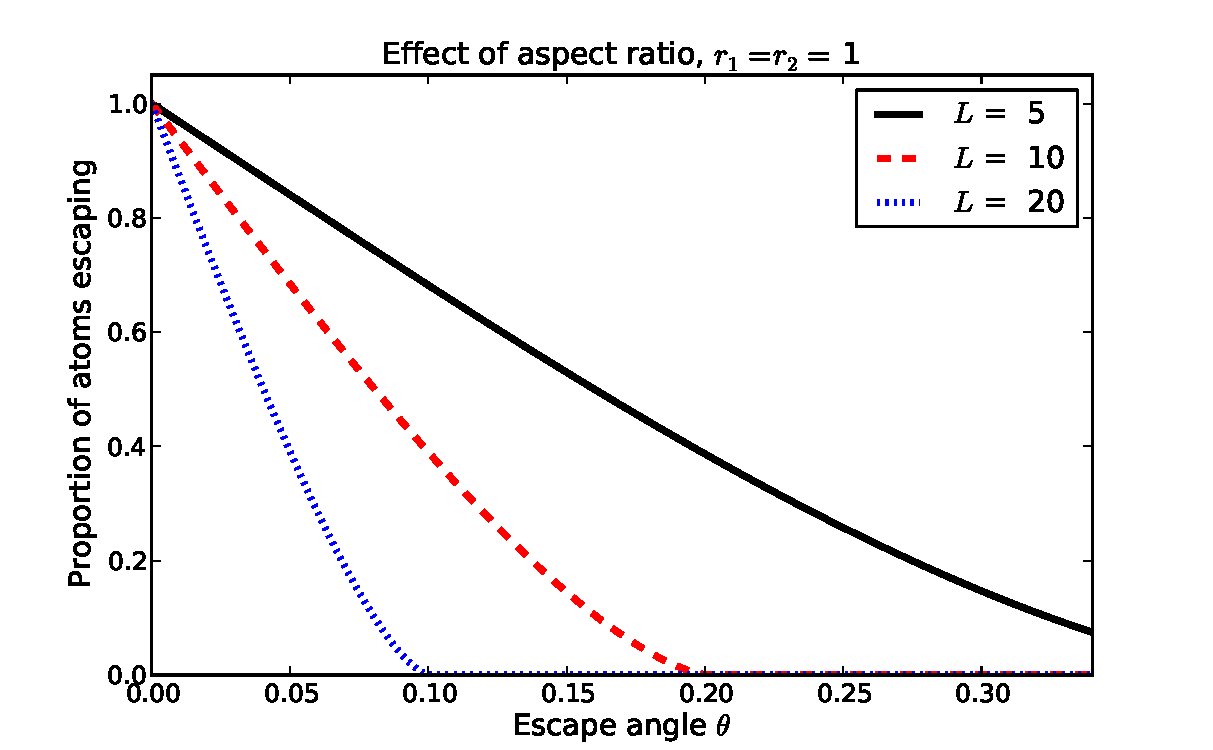
\includegraphics{pinhole_aspect.pdf}}
\caption{The effect of changing the aspect ratio of the collimator (by changing its length and keeping the pinholes the same size). Normalization is the same as on Fig. \ref{fig:entrysize}.}
\label{fig:aspect}
\end{figure}

In case of identical pinholes $r = r_1 = r_2$ Eq. \ref{eq:overlaparea} can be simplified to
\begin{equation}
A(\theta, r, L) &=& 2 r^2 \cos^{-1}\left(\frac{L \sin\theta}{2 r}\right) - \frac{1}{2} \sqrt{4r^2 - L^2\sin^2\theta}
\label{eq:simpleoverlaparea}
\end{equation}}
where Eq. \ref{eq:centreshift} was substituted for $d$.

\section{Simulation}

To check the correctness of these results the atoms behaviour was simulated for different geometries as follows:
\begin{enumerate}
\item An atom was assigned a random entry position ($x_1$, $y_2$) within the entry pinhole
\item It was also assigned a random entry angle $\theta$ (with distribution proportional to $\cos \theta$) and cylindrical angle $\phi$
\item The exit point was calculated by 
\begin{eqnarray}
x_2 &=& x_1 + L \sin\theta \cos\phi \nonumber\\
y_2 &=& y_1 + L \sin\theta \sin\phi
\end{eqnarray}
\item If the exit was within the second pinhole ($\sqrt{x_2^2 + y_2^2} < r_2$) then $\theta$ was recorded for a successful exit
\end{enumerate}
This was repeated a large number of time ($\sim$4 million atoms for each geometry). Fig. \ref{fig:simresult} shows one example result of the simulation. In all cases the theoretical numbers based on Eq. \ref{eq:outprop} were in agreement.

\begin{figure}[ht]
\centering
\resizebox{0.8\columnwidth}{!}{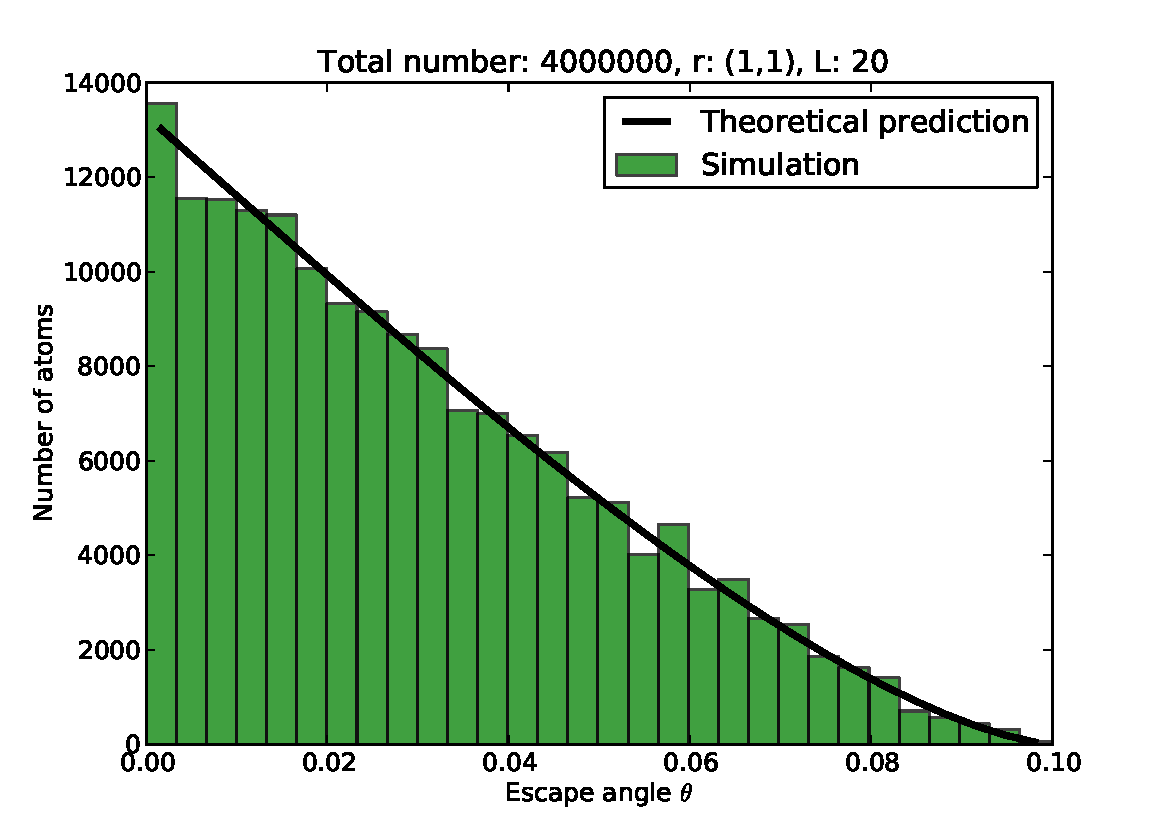
\includegraphics{pinhole_1_20.pdf}}
\caption{Simulation results of number of escaping atoms at different angles for a standard collimator geometry ($r_1 = r_2 = 1$, $L = 20$), compared to theoretical prediction based on Eq. \ref{eq:outprop}.}
\label{fig:simresult}
\end{figure}

\end{document}